\chapter{Sieć neuronowa: warstwy, konwolucja i normalizacja}\label{rozdz:siec}

\section{Z czego zbudowana jest sieć?}

Sieć neuronowa to złożenie prostych funkcji (rozdział~\ref{rozdz:zapis}); każda z nich ma kilka parametrów, które dobieramy gradientem
(rozdział~\ref{rozdz:pochodne}). Model Gen~6 używa pięciu rodzajów cegiełek: warstwy liniowej (rozdział~\ref{rozdz:wektory}), funkcji nieliniowej GELU,
konwolucji, normalizacji warstwy i połączeń resztkowych. Poznajmy je po kolei, ze sprawdzeniem na małych liczbach.

Po tym rozdziale umiesz: (i)~policzyć GELU i konwolucję jednowymiarową ręcznie, (ii)~policzyć liczbę parametrów konwolucji,
(iii)~wyznaczyć pole widzenia stosu konwolucji z dylatacją, (iv)~uzasadnić własności LayerNorm i połączenia resztkowego.

\section{Nieliniowość: po co i jaka}

Z twierdzenia~\ref{tw:mnozenie} wiemy, że dwie warstwy liniowe to jedna warstwa liniowa. Żeby głębokość coś dawała, między warstwami wstawiamy funkcję nieliniową działającą na każdą liczbę osobno.

\haslo{GELU}
\begin{definicja}[GELU]\label{def:gelu}
Niech $\Phi(z)=\tfrac12\big(1+\operatorname{erf}(z/\sqrt2)\big)$ będzie dystrybuantą rozkładu normalnego $N(0,1)$. Funkcja
$\GELU(z)=z\,\Phi(z)$ „bramkuje” wejście: mnoży je przez prawdopodobieństwo, że losowa liczba $N(0,1)$ jest mniejsza od $z$.
Dla porównania $\ReLU(z)=\max(0,z)$.
\end{definicja}

\begin{przyklad}\label{prz:gelu}
$\GELU(2)=2\cdot0{,}9772=1{,}9545$, $\GELU(1)=0{,}8413$, $\GELU(0)=0$, $\GELU(-1)=-0{,}1587$, $\GELU(-3)=-0{,}0040$.
Dla dużych dodatnich $z$ funkcja zachowuje się jak $z$, dla dużych ujemnych dąży do zera; w okolicy zera jest gładka (rys.~\ref{rys:gelu}).
\end{przyklad}

\begin{figure}[ht]
\centering
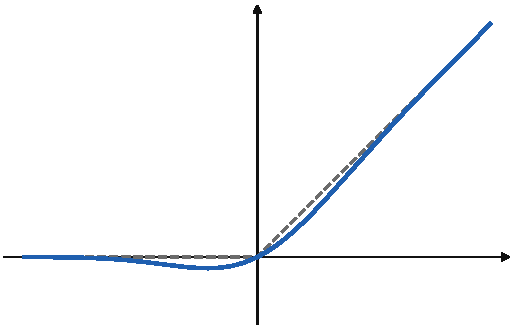
\includegraphics[width=\linewidth]{figures/gelu.pdf}
\sidecaption{GELU (niebieska) i ReLU (szara przerywana). GELU jest gładką wersją ReLU: w odróżnieniu od niego ma niewielką ujemną „zatokę” (minimum ok.\ $-0{,}17$) i nie ma ostrego załamania w zerze,
więc ma pochodną wszędzie. \label{rys:gelu}}
\end{figure}

\begin{intuicja}
ReLU wycina wszystko ujemne. GELU robi to łagodnie: małe ujemne wartości są tylko osłabiane. Przez to pochodna zmienia się płynnie i sieć uczy się stabilniej. Sam kształt nie jest świętością --- ważne jest, by funkcja była nieliniowa.
\end{intuicja}

\section{Konwolucja}

Warstwa liniowa łączy każde wejście z każdym wyjściem. Dla sygnałów, w których ten sam wzorzec może wystąpić w różnych miejscach (nuta w dowolnej klatce, wzorzec alikwotów w dowolnej wysokości), lepsza jest warstwa, która
\emph{używa tych samych wag w każdym miejscu}.

\haslo{konwolucja}
\begin{definicja}[Konwolucja jednowymiarowa]\label{def:konwolucja}
Dla sygnału $x[t]$ i \emph{jądra} $w[-r],\dots,w[r]$ (długość $k=2r+1$) wynik konwolucji z krokiem $1$ i dopełnieniem zerami to
\begin{equation}
  y[t]=b+\sum_{j=-r}^{r}w[j]\,x[t+j],
\end{equation}
przy czym $x[s]=0$ poza zakresem. \emph{Dylatacja} $d$ rozstawia próbki jądra co $d$: $y[t]=b+\sum_j w[j]\,x[t+dj]$.
\emph{Krok} (stride) $s$ oblicza wynik tylko co $s$-te $t$.
\end{definicja}

\begin{przyklad}\label{prz:konwolucja}
Sygnał $x=(1,2,3,4,5,6)$, jądro $w=(1,0,-1)$ (dla $j=-1,0,1$), $b=0$: $y[t]=x[t-1]-x[t+1]$. Wynik: $y=(-2,-2,-2,-2,-2,\,5)$.
Różnica „poprzedni minus następny” wynosi $-2$ wszędzie, gdzie sygnał rośnie liniowo; ostatnia wartość $5=x[5]-0$ pochodzi z dopełnienia zerem, które
udaje, że za końcem jest $x=0$. Takie jądro wykrywa nachylenie sygnału, czyli działa jak pochodna.
\end{przyklad}

W obrazach i widmach (dwa wymiary: czas i bin) jądro ma kształt $k_t\times k_p$ i przesuwa się w obu osiach. Jeśli każde z $C_\mathrm{we}$ kanałów wejściowych ma osobne jądro, a wyniki sumujemy do $C_\mathrm{wy}$ kanałów:

\begin{twierdzenie}[Liczba parametrów konwolucji]\label{tw:param-konw}
Konwolucja $k_t\times k_p$ z $C_\mathrm{we}$ kanałów do $C_\mathrm{wy}$ kanałów ma $C_\mathrm{we}\,C_\mathrm{wy}\,k_tk_p+C_\mathrm{wy}$ parametrów, a konwolucja \emph{głębokościowa} (osobne jądro dla każdego kanału, $C_\mathrm{we}=C_\mathrm{wy}=C$)
ma $C\,k_tk_p+C$ parametrów. Liczba ta \emph{nie zależy} od długości sygnału.
\end{twierdzenie}
\begin{pomyslDowodu}
Każdy z $C_\mathrm{wy}$ kanałów wyjściowych ma po jednym jądrze $k_t\times k_p$ dla każdego kanału wejściowego i jedno obciążenie.
\end{pomyslDowodu}
\begin{proof}
Jedno jądro ma $k_tk_p$ liczb. Kanał wyjściowy sumuje wkłady wszystkich kanałów wejściowych, więc ma $C_\mathrm{we}$ jąder i jedno obciążenie $b$.
\begin{align*}
\#\text{parametrów} &= C_\mathrm{wy}\cdot\big(C_\mathrm{we}\cdot k_tk_p+1\big) && \pow{(po kanale wyjściowym)}\\
 &= C_\mathrm{we}C_\mathrm{wy}k_tk_p+C_\mathrm{wy}. && \pow{(rozdzielność)}
\end{align*}
W wersji głębokościowej każdy kanał ma tylko jedno jądro (dla samego siebie): $C(k_tk_p+1)$. Wagi są te same dla każdego położenia, więc liczba parametrów nie rośnie z długością sygnału. To kończy dowód.
\end{proof}

\begin{naliczbach}
Trzon Gen~6: konwolucja $3\times7$ z $9$ kanałów (HCQT) do $48$: $9\cdot48\cdot21+48=9120$. Konwolucja głębokościowa $1\times5$ na $48$ kanałach: $48\cdot5+48=288$.
Konwolucja czasowa $3\times1$, $48\to48$: $48\cdot48\cdot3+48=6960$. Konwolucja $1\times1$ ($336\to48$): $336\cdot48+48=16\,176$ (to warstwa liniowa działająca w każdym miejscu osobno).
\end{naliczbach}

\begin{twierdzenie}[Konwolucja jest równoważna przesunięciom]\label{tw:rownowaznosc}
Niech $(Tx)[t]=x[t-s]$ będzie przesunięciem sygnału o $s$ w czasie. Konwolucja $C$ (bez dopełnienia, w nieskończonym sygnale) spełnia $C(Tx)=T(Cx)$.
\end{twierdzenie}
\begin{pomyslDowodu}
Wstawiamy przesunięty sygnał do definicji i przesuwamy indeks.
\end{pomyslDowodu}
\begin{proof}
\begin{align*}
(C(Tx))[t] &= b+\sum_j w[j]\,(Tx)[t+j] && \pow{(def.~\ref{def:konwolucja})}\\
 &= b+\sum_j w[j]\,x[t+j-s] && \pow{(def.\ $T$)}\\
 &= (Cx)[t-s]=(T(Cx))[t]. && \pow{(def.\ $C$ w punkcie $t-s$)}
\end{align*}
Przesunięcie wejścia o $s$ klatek przesuwa wynik o $s$ klatek, a niczego innego nie zmienia: ta sama nuta w innym momencie daje ten sam wzorzec odpowiedzi. To kończy dowód.
\end{proof}

W praktyce to właśnie dlatego konwolucja po osi binów (na osi logarytmicznej, rozdział~\ref{rozdz:alikwoty}) wykrywa ten sam wzorzec nuty o dowolnej wysokości.

\haslo{pole widzenia}
\begin{twierdzenie}[Pole widzenia]\label{tw:pole-widzenia}
Stos $n$ konwolucji w czasie z jądrami długości $k_i=2r_i+1$ i dylatacjami $d_i$ ma \emph{pole widzenia} (liczbę klatek wejścia z każdej strony, które wpływają na jedną klatkę wyjścia)
$R=\sum_{i=1}^{n}d_ir_i$.
\end{twierdzenie}
\begin{pomyslDowodu}
Indukcja po liczbie warstw: każda nowa warstwa rozszerza zbiór zależności o $d_ir_i$ klatek z każdej strony.
\end{pomyslDowodu}
\begin{proof}
Dla $n=1$: wyjście w klatce $t$ zależy od wejść w $t+d_1j$, $|j|\le r_1$, czyli od klatek odległych najwyżej o $d_1r_1$. Załóżmy, że wyjście warstwy $n-1$ w klatce $u$ zależy od wejść odległych najwyżej o $R_{n-1}$.
Wyjście warstwy $n$ w klatce $t$ zależy od wyjść warstwy $n-1$ w $u=t+d_nj$, $|j|\le r_n$, a każde z nich od wejść odległych o co najwyżej $R_{n-1}$ od $u$. Najdalsza zależność od $t$ to
\begin{align*}
|u-t|+R_{n-1}\le d_nr_n+R_{n-1}=R_n && \pow{(nierówność trójkąta)}
\end{align*}
i ta odległość jest osiągana (dla $j=\pm r_n$ i skrajnej zależności wcześniejszej, gdy odpowiednie wagi są niezerowe). Zatem $R=\sum d_ir_i$. To kończy dowód.
\end{proof}

\begin{figure*}[ht]
\centering
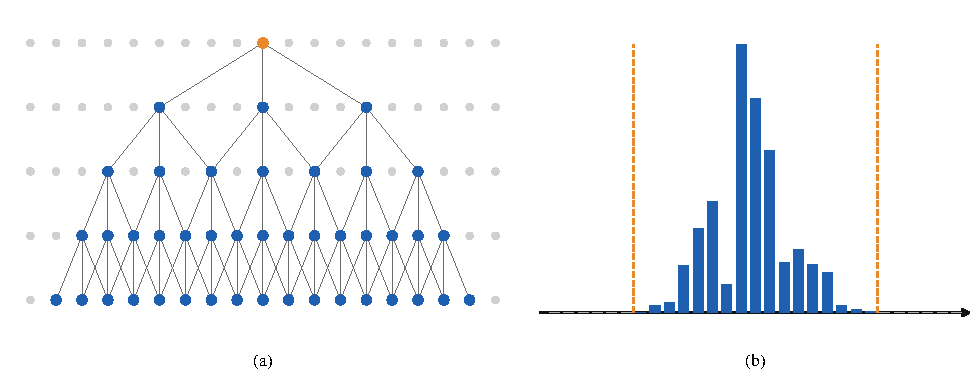
\includegraphics[width=\linewidth]{figures/pole-widzenia.pdf}
\caption{(a) Schemat czterech konwolucji czasowych z jądrem $3$ i dylatacjami $1$ (trzon), $1,2,4$ (od wejścia na dole do wyjścia na górze): pomarańczowa kropka to jedna klatka wyjścia, niebieskie to klatki wejścia, od których zależy
(zasięg $\pm8=1+1+2+4$). Z dylatacją pole widzenia rośnie wykładniczo, a nie liniowo, przy tej samej liczbie parametrów.
(b) Pomiar: moduł gradientu jednej wartości wyjścia po wejściu w funkcji odległości w klatkach dla stosu z trzonem $3\times7$ i trzema blokami z dylatacjami $1,2,4$ (losowe wagi, PyTorch): gradient jest niezerowy dokładnie dla $|t|\le8=1+(1+2+4)$ (niebieskie) i zerowy poza (szare).}
\label{rys:pole-widzenia}
\end{figure*}

\begin{przyklad}[Pole widzenia bloków Gen~6]\label{prz:pole-gen6}
Trzon ma jądro $3$ w czasie ($r=1$, $d=1$) i trzy bloki mają jądro $3$ z $d=1,2,4$: $R=1+(1+2+4)=8$ klatek, czyli $\pm8\cdot23{,}2\ms=\pm186\ms$. Pomiar na prawdziwym stosie (rys.~\ref{rys:pole-widzenia}b) potwierdza $\pm8$.
\end{przyklad}

\section{Normalizacja warstwy i połączenia resztkowe}

\haslo{LayerNorm}
\begin{definicja}[LayerNorm]\label{def:ln}
Dla wektora $\vect z\in\R^D$ niech $\mu=\frac1D\sum z_i$ i $\sigma^2=\frac1D\sum(z_i-\mu)^2$. \emph{Normalizacja warstwy} to
$\LN(\vect z)_i=\gamma_i\,\dfrac{z_i-\mu}{\sqrt{\sigma^2+\varepsilon}}+\beta_i$, gdzie $\gamma,\beta\in\R^D$ są uczone ($\gamma=1,\beta=0$ na starcie), a $\varepsilon=10^{-5}$ chroni przed dzieleniem przez zero.
\end{definicja}

\begin{przyklad}\label{prz:ln}
Dla $\vect z=(1,2,3,6)$: $\mu=3$, $\sigma^2=(4+1+0+9)/4=3{,}5$, $\sigma=1{,}871$. Wynik (przy $\gamma=1$, $\beta=0$, $\varepsilon\to0$): $(-1{,}069;\,-0{,}535;\,0;\,1{,}604)$ ma średnią $0$ i wariancję $1$.
\end{przyklad}

\begin{twierdzenie}[Niezmienniczość LayerNorm]\label{tw:ln}
Dla $\varepsilon=0$, $\gamma=1$, $\beta=0$ i dowolnych $a>0$, $c\in\R$: $\LN(a\vect z+c\vect 1)=\LN(\vect z)$.
\end{twierdzenie}
\begin{pomyslDowodu}
Skalowanie i przesunięcie zmieniają średnią i odchylenie dokładnie w taki sposób, że licznik i mianownik skracają się.
\end{pomyslDowodu}
\begin{proof}
Dla $\vect z'=a\vect z+c\vect1$: $\mu'=a\mu+c$ oraz
\begin{align*}
\sigma'^2 &= \frac1D\sum(az_i+c-a\mu-c)^2=a^2\sigma^2 && \pow{(wyrazy $c$ się znoszą)}\\
\frac{z'_i-\mu'}{\sigma'} &= \frac{a(z_i-\mu)}{a\sigma}=\frac{z_i-\mu}{\sigma}. && \pow{($a>0$, więc $\sqrt{a^2}=a$)}
\end{align*}
Obie strony równości są więc identyczne. To kończy dowód.
\end{proof}

W zwykłym języku: LayerNorm usuwa informację o skali i przesunięciu wektora cech i zostawia tylko jego „kształt”; wymusza to stabilny rozmiar liczb płynących przez sieć. Wady: nie działa na wektorach stałych ($\sigma=0$; stąd $\varepsilon$).

\haslo{połączenie resztkowe}
\begin{definicja}[Połączenie resztkowe]\label{def:residual}
Blok z połączeniem resztkowym liczy $\vect y=\vect x+F(\vect x)$, gdzie $F$ to dowolna warstwa lub kilka warstw (rys.~\ref{rys:blok}).
\end{definicja}

\begin{twierdzenie}[Gradient przez połączenie resztkowe]\label{tw:residual}
Dla $\vect y=\vect x+F(\vect x)$ macierz pochodnych (jakobian) to $\dfrac{\partial\vect y}{\partial\vect x}=I+\dfrac{\partial F}{\partial\vect x}$. Dla stosu $L$ takich bloków
\begin{equation}
  \frac{\partial\vect y_L}{\partial\vect x}=\prod_{l=1}^{L}\big(I+J_l\big)=I+\sum_{l}J_l+(\text{wyrazy wyższych rzędów w }J).
\end{equation}
\end{twierdzenie}
\begin{pomyslDowodu}
Pochodna sumy to suma pochodnych, a pochodna $\vect x$ po $\vect x$ to macierz jednostkowa; dla stosu mnożymy jakobiany (reguła łańcuchowa).
\end{pomyslDowodu}
\begin{proof}
Z liniowości pochodnej $\partial(\vect x+F(\vect x))/\partial\vect x=\partial\vect x/\partial\vect x+\partial F/\partial\vect x=I+J$. Dla stosu reguła łańcuchowa daje iloczyn jakobianów kolejnych bloków. Rozwijając iloczyn $(I+J_L)\cdots(I+J_1)$ otrzymujemy $I$ (wybór składnika $I$ z każdego nawiasu), plus $J_l$ (jeden nawias daje $J$), plus iloczyny dwóch i więcej $J$. Człon $I$ nie zależy od $F$. To kończy dowód.
\end{proof}

W zwykłym języku: nawet jeśli $F$ ma bardzo małe pochodne, sygnał uczący przepływa przez „autostradę” $I$ i nie znika. Dzięki temu można ułożyć wiele bloków bez ryzyka, że gradient wygaśnie po drodze.

\begin{naliczbach}
Dla skalarnej $F(x)=0{,}01x$ i $L=50$ bloków: z połączeniem $\prod(1+0{,}01)=1{,}01^{50}=1{,}645$, bez niego $\prod0{,}01=10^{-100}$. Gradient bez autostrady byłby praktycznie zerem.
\end{naliczbach}

\begin{figure}[ht]
\centering
\begin{tikzpicture}[>=Stealth,node distance=6mm]
  \node[blok,minimum width=14mm] (x) {$\vect x$};
  \node[blok,minimum width=16mm,right=of x] (ln) {$\LN$};
  \node[blok,minimum width=16mm,right=of ln] (f) {$F$};
  \node[blok,minimum width=14mm,right=of f] (drop) {$\Drop$};
  \node[wezel,right=8mm of drop] (plus) {$+$};
  \node[right=7mm of plus] (y) {$\vect y$};
  \draw[wektor] (x)--(ln); \draw[wektor] (ln)--(f); \draw[wektor] (f)--(drop); \draw[wektor] (drop)--(plus); \draw[wektor] (plus)--(y);
  \draw[wektor] (x.north) -- ++(0,6mm) -| (plus.north);
\end{tikzpicture}
\sidecaption{Blok resztkowy typu „pre-norm”, jak w warstwach Gen~6: wejście $\vect x$ jest normalizowane (LN), przechodzi przez $F$ (konwolucja albo uwaga) i dropout, a następnie dodawane do niezmienionego $\vect x$ (górna ścieżka). Wynik: $\vect y=\vect x+\Drop(F(\LN(\vect x)))$. \label{rys:blok}}
\end{figure}

\haslo{dropout}
\begin{definicja}[Dropout]\label{def:dropout}
W uczeniu \emph{dropout} z prawdopodobieństwem $\rho$ zeruje każdą współrzędną wektora, a pozostałe mnoży przez $\frac1{1-\rho}$. Przy wnioskowaniu nie robi nic.
\end{definicja}

\begin{wniosek}[Dropout nie zmienia średniej]\label{wn:dropout}
Dla $\vect x$ ustalonego, $\Exp[\Drop(\vect x)]=\vect x$.
\end{wniosek}
\begin{proof}
Dla jednej współrzędnej $x_i$ wynik wynosi $0$ z prawdopodobieństwem $\rho$ i $x_i/(1-\rho)$ z prawdopodobieństwem $1-\rho$. Stąd
\begin{align*}
\Exp[\Drop(x_i)] &= \rho\cdot0+(1-\rho)\cdot\frac{x_i}{1-\rho}=x_i. && \pow{(definicja wartości oczekiwanej)}
\end{align*}
Skalowanie przez $\frac{1}{1-\rho}$ sprawia, że przy wnioskowaniu (bez dropoutu) liczby mają ten sam rząd wielkości co w uczeniu. Gen~6 używa $\rho=0{,}1$. To kończy dowód.
\end{proof}

\begin{pulapka}
LayerNorm i dropout zachowują się inaczej w uczeniu i wnioskowaniu (dropout) lub zależą od wymiaru (LayerNorm liczy po cechach jednego punktu, nie po paczce). Błąd typowy: zapomnieć wywołać \texttt{model.eval()} przed przewidywaniem; sieć wciąż losowo zeruje cechy i wyniki są inne przy każdym uruchomieniu.
\end{pulapka}

\section*{Podsumowanie}
\begin{itemize}
\item Między warstwami liniowymi stawiamy nieliniowość GELU $=z\Phi(z)$.
\item Konwolucja używa tych samych wag w każdym miejscu; liczba parametrów to $C_\mathrm{we}C_\mathrm{wy}k_tk_p+C_\mathrm{wy}$ i nie zależy od długości sygnału (tw.~\ref{tw:param-konw}); jest równoważna przesunięciom (tw.~\ref{tw:rownowaznosc}).
\item Pole widzenia stosu konwolucji: $R=\sum d_ir_i$ (tw.~\ref{tw:pole-widzenia}); dla bloków Gen~6 $R=8$ klatek.
\item LayerNorm usuwa skalę i przesunięcie wektora cech (tw.~\ref{tw:ln}).
\item Połączenie resztkowe $\vect x+F(\vect x)$ zachowuje gradient (tw.~\ref{tw:residual}); dropout nie zmienia średniej (wn.~\ref{wn:dropout}).
\end{itemize}

\begin{sprawdz}
\begin{enumerate}
\item Policz konwolucję $x=(2,0,1,3)$ z jądrem $w=(1,2,1)$ (dla $j=-1,0,1$, $b=0$) i dopełnieniem zerami.
\item Ile parametrów ma konwolucja $5\times5$ z $16$ do $32$ kanałów? A głębokościowa $5\times5$ na $32$ kanałach?
\item Stos czterech konwolucji z jądrem $3$ i dylatacjami $1,2,4,8$. Jakie jest pole widzenia? Ile wynosiłoby bez dylatacji?
\item Policz $\LN(\vect z)$ dla $\vect z=(4,4,8)$ ($\gamma=1,\beta=0,\varepsilon\to0$).
\end{enumerate}
\end{sprawdz}

\subsection*{Rozwiązania}
\begin{enumerate}
\item $y[0]=1\cdot0+2\cdot2+1\cdot0=4$ (bo $x[-1]=0$); $y[1]=1\cdot2+2\cdot0+1\cdot1=3$; $y[2]=1\cdot0+2\cdot1+1\cdot3=5$; $y[3]=1\cdot1+2\cdot3+1\cdot0=7$. Wynik $(4,3,5,7)$.
\item $16\cdot32\cdot25+32=12\,832$; głębokościowa: $32\cdot25+32=832$.
\item $R=1+2+4+8=15$ klatek z każdej strony; bez dylatacji $R=4$.
\item $\mu=16/3=5{,}333$; $\sigma^2=\frac13\big(2\cdot1{,}778+7{,}111\big)=3{,}556$, $\sigma=1{,}886$. Wynik: $(-0{,}707;\,-0{,}707;\,1{,}414)$.
\end{enumerate}
